\documentclass[10pt, conference, compsocconf,hyphens]{IEEEtran}
\usepackage{mathptmx}
\usepackage{amsmath}
%\usepackage{mathtools}
\usepackage{courier}
\usepackage[scaled=.92]{helvet}

\usepackage[pdfborder={0 0 0},bookmarks=false,breaklinks,draft]{hyperref}

\usepackage{graphicx}
\usepackage{color}
\usepackage{xspace}
\usepackage{listings}
\usepackage{booktabs,tabularx}
\usepackage[numbers,sort]{natbib}
\usepackage{ragged2e}
\usepackage{tikz}
\usepackage{dcolumn}
\usepackage{dsfont}
\usepackage{pdfpages}
\usepackage{listings}

\lstset{language=C,basicstyle=\ttfamily,xleftmargin=2em}

\iffalse % Change to \iffalse for submission
\usepackage{datetime}
\usepackage{fancyhdr}
\fancypagestyle{IEEEtitlepagestyle}{%
\fancyhead{}
\fancyfoot[L]{\textcolor{red}{\bfseries DRAFT}}
\fancyfoot[C]{\thepage}
\fancyfoot[R]{\textcolor{red}{\bfseries\currenttime\ \today}}
\renewcommand\headrulewidth{0pt}
\renewcommand\footrulewidth{0pt}}
\pagestyle{IEEEtitlepagestyle}
\fi
\usepackage{flushend}

\usepackage[binary-units]{siunitx}
\usepackage{subcaption}
\usepackage{multirow}
%\usepackage[title,header]{appendix}
\usepackage{lipsum}
\usepackage[absolute]{textpos}
\usepackage[T1]{fontenc}

\providecommand{\st}{\ensuremath{\mathrm{\ s.t.\ }}}

\providecommand{\bagmap}{\texttt{bagmap}}
\providecommand{\bagsum}{\texttt{bagsum}}
\providecommand{\bagsize}{\texttt{bagsize}}
\providecommand{\bagsplit}{\texttt{bagsplit}}

\providecommand{\lone}{\ensuremath{\ell{}_1}}

\hyphenation{white-list}

% taken from hs's mary.tex, and tracing back to knuth.
\def\dash---{\kern.16667em---\penalty\exhyphenpenalty\hskip.16667em\relax}

% C++ macro from john mitchell
\def\CC{C\raise.22ex\hbox{{\footnotesize +}}\raise.22ex\hbox{\footnotesize +}\xspace}

% Make URLs linebreak better (hat-tip alexras)
  % A sequence of BigBreaks will be treated as one break, so it will only be able to break after ://
  \renewcommand{\UrlBigBreaks}{\do\:\do\/}
  % (Less aggressive) Treat both / and - as breakable characters (don't know why this does something different than hyphens in the package declaration, but it does)
  \renewcommand{\UrlBreaks}{\do\/\do\-}
  % (More aggressive) Any letter and / are treated as breakable characters
  \renewcommand{\UrlBreaks}{\do\/\do\a\do\b\do\c\do\d\do\e\do\f\do\g\do\h\do\i\do\j\do\k\do\l\do\m\do\n\do\o\do\p\do\q\do\r\do\s\do\t\do\u\do\v\do\w\do\x\do\y\do\z\do\A\do\B\do\C\do\D\do\E\do\F\do\G\do\H\do\I\do\J\do\K\do\L\do\M\do\N\do\O\do\P\do\Q\do\R\do\S\do\T\do\U\do\V\do\W\do\X\do\Y\do\Z}

\lstdefinelanguage{JavaScript}{
  morekeywords={typeof, new, true, false, catch, function, return, null, catch, switch, var, if, in, while, do, else, case, break},
  morecomment=[s]{/*}{*/},
  morecomment=[l]//,
  morestring=[b]'',
  morestring=[b]'
}

\lstdefinelanguage{HTML5}{
        language=html,
        sensitive=true,
        alsoletter={<>=-},
        otherkeywords={
        % HTML tags
        <feConvolveMatrix, />
        },
        ndkeywords={
        % General
        =,
        % HTML attributes
        charset=, id=, width=, height=, in=, order=, edgeMode=, kernelMatrix=, preserveAlpha=,
        % CSS properties
        border:, transform:, -moz-transform:, transition-duration:, transition-property:, transition-timing-function:,
        },
        morecomment=[s]{<!--}{-->},
        tag=[s]
}

\lstset{%
    % Code
    language=HTML5,
    alsolanguage=JavaScript,
    showstringspaces=false,
    extendedchars=true,
    breaklines=true
 }

\providecommand{\setjmp}{\texttt{setjmp}}
\providecommand{\longjmp}{\texttt{longjmp}}

% Alter some LaTeX defaults for better treatment of figures:
    % See p.105 of "TeX Unbound" for suggested values.
    % See pp. 199-200 of Lamport's "LaTeX" book for details.
    %   General parameters, for ALL pages:
    \renewcommand{\topfraction}{0.9}    % max fraction of floats at top
    \renewcommand{\bottomfraction}{0.8} % max fraction of floats at bottom
    %   Parameters for TEXT pages (not float pages):
    \setcounter{topnumber}{2}
    \setcounter{bottomnumber}{4}
    \setcounter{totalnumber}{6}         % 2 may work better
    \setcounter{dbltopnumber}{2}        % for 2-column pages
    \renewcommand{\dbltopfraction}{0.9} % fit big float above 2-col. text
    \renewcommand{\textfraction}{0.07}  % allow minimal text w. figs
    %   Parameters for FLOAT pages (not text pages):
    \renewcommand{\floatpagefraction}{0.7}  % require fuller float pages
    % N.B.: floatpagefraction MUST be less than topfraction !!
    \renewcommand{\dblfloatpagefraction}{0.7} % require fuller float pages


\setlength{\TPHorizModule}{30mm}
\setlength{\TPVertModule}{\TPHorizModule}
\textblockorigin{10mm}{10mm}

\newcolumntype{C}[1]{>{\centering\let\newline\\\arraybackslash\hspace{0pt}}m{#1}}

% get rid of that stupid box on the first page.
\makeatletter
\def\@copyrightspace{}
\makeatother

% Support cool highlighting boxes in lstlisting (from
% http://tex.stackexchange.com/questions/15237/highlight-text-in-code-listing-while-also-keeping-syntax-highlighting)
\makeatletter
\newenvironment{btHighlight}[1][]
{\begingroup\tikzset{bt@Highlight@par/.style={#1}}\begin{lrbox}{\@tempboxa}}
{\end{lrbox}\bt@HL@box[bt@Highlight@par]{\@tempboxa}\endgroup}

\newcommand\todo[1]{\textcolor{red}{TODO:#1}}

\newcommand\btHL[1][]{%
  \begin{btHighlight}[#1]\bgroup\aftergroup\bt@HL@endenv%
}
\def\bt@HL@endenv{%
  \end{btHighlight}%
  \egroup
}
\newcommand{\bt@HL@box}[2][]{%
  \tikz[#1]{%
    \pgfpathrectangle{\pgfpoint{1pt}{0pt}}{\pgfpoint{\wd #2}{\ht #2}}%
    \pgfusepath{use as bounding box}%
    \node[anchor=base west, fill=orange!30,outer sep=0pt,inner xsep=1pt, inner ysep=0pt, rounded corners=3pt, minimum height=\ht\strutbox+1pt,#1]{\raisebox{1pt}{\strut}\strut\usebox{#2}};
  }%
}
\lstdefinestyle{Chighlight}{
    language={C},basicstyle=\ttfamily,
    moredelim=**[is][\btHL]{`}{`},
    moredelim=**[is][{\btHL[fill=green!30,draw=red,dashed,thin]}]{@}{@},
}
\makeatother


% support aligning a table column on .
\newcolumntype{d}[1]{D{.}{.}{#1} }

\def\sharedaffiliation{
\end{tabular}
\begin{tabular}{c}}
\begin{document}


\title{802.11ac performance in 802.11a/b/g/n dominated environments}

\author{
\IEEEauthorblockN{David Kohlbrenner, Jake Maskiewicz, Sean Hamilton}
\IEEEauthorblockA{
University of California, San Diego\\
}
}


\clubpenalty=10000
\widowpenalty=10000

\maketitle

%\section{Schedule}

%A schedule, specifying concretely what you intend to have accomplished by each
%of the two milestones below as well as for the final report/presentation. It is
%perfectly acceptable if the final deliverable is not a completion of the
%project---which, if successful, some members of the group may wish to continue
%after the term ends---but it does need to be something that can be clearly
%demonstrated/evaluated/graded.

Our original goals have (as we discussed) had to change. This will outline (briefly) what we hope to have done for the presentation and talk.
Obviously its less than we would have preferred, but we have less time than we would've liked to run these experiments.

\begin{enumerate}
\item Test throughput as a function of distance for the new 80MHz bandwidth and compare to the 20/40Mhz bandwidth options that were defined in 802.11g and n standard
\item Provide a theoretical analysis of throughput for 160Mz channel bandwidth as a function of distance (Our equipment doesn't support 160MHz)
\item Test throughput for the newer modulation 256QAM modulation scheme and the two accompanying FEC codings (MCS 8 and 9)
\item Test and analyze the throughput and parallelism of MU-MIMO that is supported in 802.11ac
\end{enumerate}

\section{Resources}

At current, we have access to two 802.11AC WAPs (although one is
running the internet at Sean's house, and can't be moved too
frequently). Additionally, we have a number of devices that can act as
802.11AC clients, including a Macbook Pro, a Microsoft Surface Pro 3,
and two mobile devices, an iPhone 6 and an Android OnePlus
One. Through these devices would be sufficient to test a small level
of congestion for two networks, we would like to test congestion
across multiple networks from several WAPs, so additional 802.11AC
capable WAPs would be required. Additionally, if we wish to test
multiple beam-forming setups, we will require more APs, since none of
our clients (to the best of our knowledge) support outbound
beam-forming. To measure interference between 802.11b/g/n and AC, we
have several g/n APs available, as well as testing at UCSD in various
buildings.

Ideally, we would purchase at least one USB 802.11AC dongle
(\$20-\$50) and another 802.11AC access point (\$50-\$200). This would
allow us to test interference from multiple 802.11AC networks on each
other, as well as on 802.11b/g/n. We are also interested in working
with some of the 802.11 test-bed hardware used in Patrick Verkaik's
work (ie \cite{kandula2009detailed}) if it is available. One of our
first tasks will be to evaluate what is actually feasible with the
equipment we end up with.

\section{Tools}

We have decided to use iperf3 (both TCP and UDP) to measure bandwidth
and characteristics between machines in our network. Initial tests
were run with one machine hardwired via ethernet to the router running
an iperf server, and the other machine wirelessly connected as an
iperf client. In subsequent tests, we were able to install iperf
directly on the router, and run the server from there. There is some
concern that this will degrade the performance of the router, and we
intend to measure the difference between the two setups to determine
if that is the case.

\section{Results}
\todo{results}
\begin{figure}[!h]
\centering
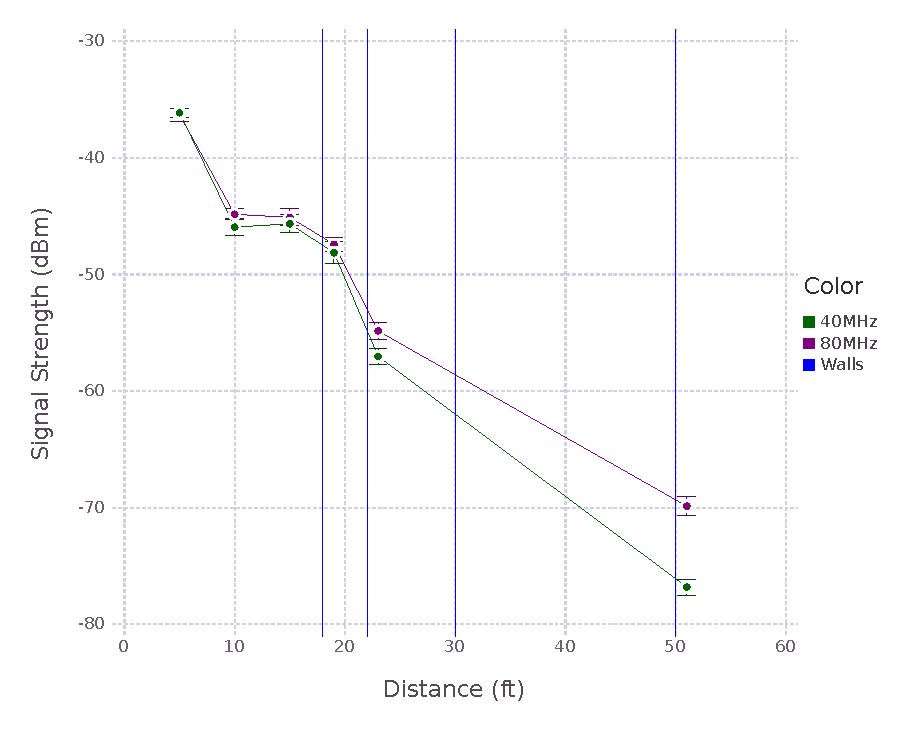
\includegraphics[width=0.5\textwidth]{figures/Intel_Inside_Beamformed}
\caption{Intel Indoor Signal}
\end{figure}

\section{Schedule}

%A schedule, specifying concretely what you intend to have accomplished by each
%of the two milestones below as well as for the final report/presentation. It is
%perfectly acceptable if the final deliverable is not a completion of the
%project---which, if successful, some members of the group may wish to continue
%after the term ends---but it does need to be something that can be clearly
%demonstrated/evaluated/graded.

\subsection{Feb. 19}
\begin{enumerate}
\item All hardware in-hand, cataloged, and tested. We will have documented all the listed features and performance of all devices we will be testing.
\item A testing suite, with associated metrics and benchmarking tools.
\item Preliminary results from running the testing tools on our 802.11ac and 802.11 g/n networks in isolation (no notable RF interference)
\end{enumerate}

\subsection{Mar. 5}
\begin{enumerate}
\item Testing results from interference of 802.11ac and g/n networks in both RF and spatial interference
\item Testing results for beamforming/spatial stream effects on interference
\end{enumerate}
This is basically all of our data collection near
complete. Hopefully. There is enough time after this that if some
parts slip we can continue tests.

\subsection{Final}
Full data on interference between 802.11ac and 802.11b/g/n networks. This will include:
\begin{enumerate}
\item Baseline data of what our hardware is capable of in isolation
\item 802.11ac performance degradation in varying levels of 802.11b/g/n traffic
\item 802.11b/g/n performance degradation in the presence of 802.11ac
\item Above two, but with 802.11ac using spatial streams/beamforming
\item Analysis of our results, based on both previous works (see
  related work) and on what level of introspection we are able to
  obtain during the project.
\end{enumerate}

I use 802.11b/g/n in this, since we are certain to use n, but are
unsure if we will have time to do any meaningful testing comparing all
802.11 consumer technologies.

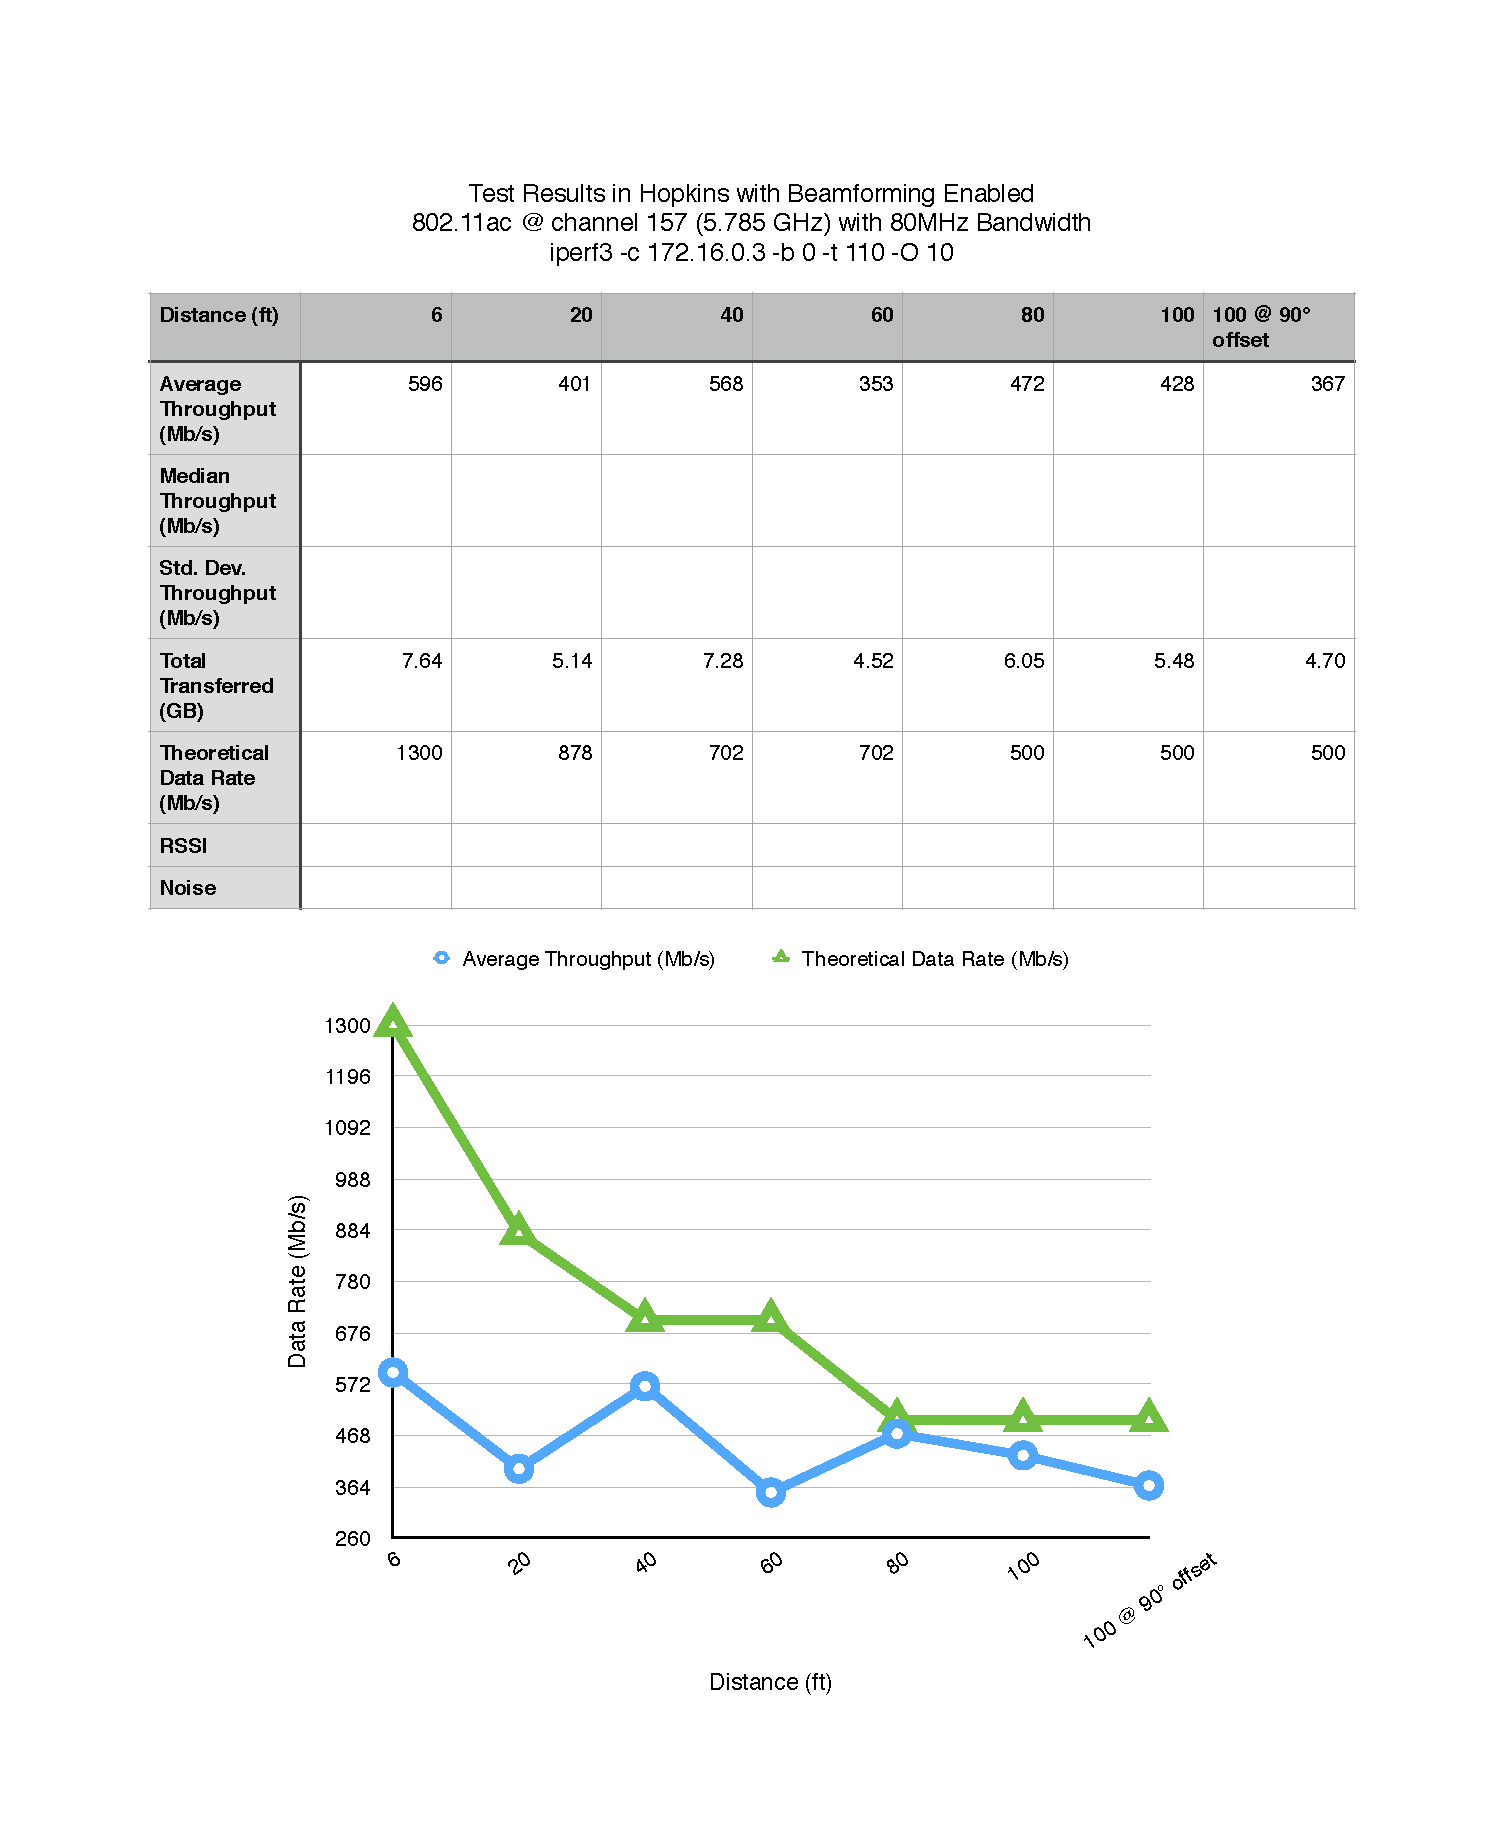
\includepdf{partial_results.pdf}

%{\small
%\bibliographystyle{IEEEtranSN}
%\bibliography{acprogress}
%}

\typeout{}

\end{document}
